% Created 2022-09-29 Thu 19:34
% Intended LaTeX compiler: pdflatex
\documentclass[11pt]{article}
\usepackage[utf8]{inputenc}
\usepackage[T1]{fontenc}
\usepackage{graphicx}
\usepackage{longtable}
\usepackage{wrapfig}
\usepackage{rotating}
\usepackage[normalem]{ulem}
\usepackage{amsmath}
\usepackage{amssymb}
\usepackage{capt-of}
\usepackage{hyperref}
\author{Shayan Naqvi}
\date{\today}
\title{Chemistry}
\hypersetup{
 pdfauthor={Shayan Naqvi},
 pdftitle={Chemistry},
 pdfkeywords={},
 pdfsubject={},
 pdfcreator={Emacs 27.1 (Org mode 9.6)}, 
 pdflang={English}}
\begin{document}

\maketitle
\tableofcontents

\section{Bonding}
\label{sec:org28b644c}
\subsection{Ionic Bonding}
\label{sec:org5a51af9}
Bonding via the transfer of electrons.
\subsection{Covalent Bonding}
\label{sec:org35d83dc}
Bonding via the sharing of electrons.
\subsection{Metallic Bonding}
\label{sec:org84e01bc}
Bonding between metallic ions and free electrons.
\subsection{Number of bonds}
\label{sec:org819ec1e}
\begin{enumerate}
\item C = 4
\item N = 3
\item O = 2
\item H = 1
\item Halogens = 1
\end{enumerate}
\section{Identification}
\label{sec:org131db2f}
\subsection{Identification of cations}
\label{sec:org6b5cb5f}
\begin{center}
\begin{tabular}{lllll}
 & Sodium Hydroxide, \(NaOH (aq)\) &  & Aqueous Ammonia, \(NH_3 (aq)\) & \\
Cation & On addition of a few drops & On addition of excess & On addition of a few drops & On addition of excess\\
\hline
Zinc, \(Zn^{2+}\) & White precipitate & Colourless solution (precipitate dissolves in excess) & White precipitate & Colourless solution (precipitate dissolves in excess)\\
Aluminium, \(Al^{3+}\) & White precipitate & Colourless solution (precipitate dissolves in excess) & White precipitate & Precipitate does not dissolve in excess (insoluble precipitate)\\
Lead(II), \(Pb^{2+}\) & White precipitate & Colourless solution (precipitate dissolves in excess) & White precipitate & Precipitate does not dissolve in excess (insoluble precipitate)\\
Calcium, \(Ca^{2+}\) & White precipitate & Precipitate does not dissolve in excess (insoluble precipitate) & No precipitate & No precipitate\\
Copper(II), \(Cu^{2+}\) & Light blue precipitate & Precipitate does not dissolve in excess (insoluble precipitate) & Light blue precipitate & Deep blue solution (soluble precipitate)\\
Iron(II), \(Fe^{2+}\) & Green precipitate & Precipitate does not dissolve in excess (insoluble precipitate) & Green precipitate & Precipitate does not dissolve in excess (insoluble precipitate)\\
Iron(III), \(Fe^{3+}\) & Reddish-brown precipitate & Precipitate does not dissolve in excess (insoluble precipitate) & Reddish-brown precipitate & Precipitate does not dissolve in excess (insoluble precipitate)\\
Ammonium, \(NH_4^+\) & No precipitate. However, if heated, ammonia gas is released, which turns \textbf{moist red litmus paper blue}. & No change is observed & - & -\\
\end{tabular}
\end{center}
\subsection{Identification of anions}
\label{sec:org4b153cd}
\begin{center}
\begin{tabular}{lll}
Anion & Test & Observation(s)\\
\hline
Carbonate, \(CO_3^{2-}\) & Addition of dilute hydrochloric acid, (\(HCl\)). Pass the gas released into limewater. & 1. Observation of effervescence.\\
 &  & 2. The gas released forms a white precipitate with limewater.\\
 &  & 3. Carbon dioxide gas is given off.\\
Nitrate, \(NO_3^-\) & Addition of sodium hydroxide, \(NaOH\), and proceed to add a piece of aluminium foil. Warm the mixture. Test the gas given off with a piece of moist red litmus paper. & 1. Observation of effervescence.\\
 &  & 2. The moist red litmus paper turns blue.\\
 &  & 3. Ammonia gas is given off.\\
Sulfate, \(SO_4^{2-}\) & Addition of dilute nitric acid, \(HNO_3\). Proceed to add a solution of barium nitrate, \(Ba(NO_3)_2\). & A white precipitate of barium sulfate is formed.\\
Chloride, \(Cl^{-}\) & Addition of dilute nitric acid, \(HNO_3\). Proceed to add a silver nitrate solution, \(AgNO_3\). & A white precipitate of silver chloride is formed.\\
Iodide, \(I^-\) & Addition of dilute nitric acid, \(HNO_3\), then silver nitrate, \(AgNO_3\). & A yellow precipitate of silver iodide is formed.\\
\end{tabular}
\end{center}
\subsection{Identification of gases}
\label{sec:org5a34f60}
\begin{center}
\begin{tabular}{llll}
Gas & Colour and odour & Test & Observation(s)\\
\hline
Hydrogen, \(H_2\) & Colourless and odourless & Lighted splint (at the mouth of the test tube) & The lighted splint is extinguished with a 'pop' sound\\
Oxygen, \(O_2\) & Colourless and odourless & Glowing splint (into the test tube) & The glowing splint if rekindled (catches fire again)\\
Carbon dioxide, \(CO_2\) & Colourless and odourless & Bubble the gas through limewater & A white precipitate is formed, which dissolves into limewater, giving it a milky colour (limewater turns milky)\\
--- & --- & --- & ---\\
Chlorine & Greenish-yellow and pungent smell & Moist blue litmus paper at the mouth of the test tube & The moist blue litmus turns blue and is then bleached\\
Sulfur dioxide, \(SO_2\) & Colourless and pungent smell & Fiter paper soaked in acidified \(KMnO_4\) (potassium manganate(VII) at the mouth of the test tube) & The purple acidified \(KMnO_4\) turns colourless\\
Ammonia, \(NH_3\) & Colourless and pungent smell & Moist red litmus paper at the mouth of the test tube & The moist red litmus turns blue\\
\end{tabular}
\end{center}
\subsection{Identification of water}
\label{sec:orgb5c8f72}
\begin{center}
\begin{tabular}{ll}
Test & Observation\\
\hline
Heat the sample in a test tube. Place a piece of cobalt(II) chloride paper at the mouth of the test tube. & Cobalt(II) chloride paper changes from blue to pink.\\
Add a few drops of the sample to some anhydrous copper(II) sulfate. & Anydrous copper(II) sulfate changes from white to blue.\\
\end{tabular}
\end{center}
\section{Redox reactions}
\label{sec:org33dda13}
\subsection{Oxidation}
\label{sec:org1305b44}
Oxidation is,
\begin{enumerate}
\item the gain of oxygen during a chemical reaction
\item an increase in oxidation state
\item the loss of hydrogen during a chemical reaction
\item the loss of electrons during a chemical reaction
\end{enumerate}
\subsubsection{Examples}
\label{sec:orgadd6a07}
\begin{itemize}
\item \(S(s) + O_2(g) --> SO_2(g)\) (sulfur has been oxidised to sulfur dioxide)
\item \(H_2S(g) + Cl_2 --> S(s) + 2HCl(g)\) (hydrogen sulfide has lost hydrogen and has oxidised to sulfur)
\item \(Mg --> Mg^{2+} + 2e^-\) (magnesium has lost electrons and has been oxidised)
\end{itemize}
\subsubsection{Oxidation state}
\label{sec:org74c5360}
Oxidation state refers to the hypothetical charge an element/atom would have if it was an ion in a compound.
\begin{enumerate}
\item Determining an oxidation state
\label{sec:org11c3bf3}
\begin{center}
\begin{tabular}{lll}
Rule & Example(s) & Oxidation state\\
\hline
The oxidation state of an element (on its own) is zero. & \(Cu\) & 0\\
The oxidation state of a simple ion is the same as its charge. & \(Li^+, O^{-2}\) & \(Li^+=+1\), \(O^{2-}=-2\)\\
Some elements have a fixed oxidation state in their compounds. & Elements from group 1, group 2, hydrogen in most compounds, oxygen i most compounds & group 1 = +1, group 2 = +2, hydrogen = +1, oxygen = -2\\
The oxidation states of the elements/atoms in a compounds sum to zero. & \(MgO --> +2 + (-2) = 0\), \(K_2O --> 2(+1) + (-2) = 0\) & 0 for both examples\\
The sum of oxidation states of a polyatomic ion (e.g., \(OH^-\)) is the same as the charge on the ion & \(OH^- --> -2 + 1 = -1\) & -1\\
\end{tabular}
\end{center}
\end{enumerate}
\subsection{Reduction}
\label{sec:org8f3e18a}
Reduction is,
\begin{enumerate}
\item the loss of oxygen during a chemical reaction
\item a decrease in oxidation state
\item the gain of hydrogen during a chemical reaction
\item the gain of electrons during a chemical reaction
\end{enumerate}
\subsubsection{Examples}
\label{sec:orgc301ad1}
\begin{itemize}
\item \(2Al(s) + 3CuO(s) --> Al_2O_3(s) + 3Cu(l)\) (copper oxide has been reduced to copper)
\item \(H_2(g) + Cl_2(g) --> S(s) + 2HCl(g)\) (chlorine has gained hydrogen and has thereby been reduced to hydrochloric acid)
\item \(Cl_2 + 2e^- --> 2Cl^-\) (chlorine has gained electrons and has been reduced)
\end{itemize}
\subsection{Identifying a redox reaction}
\label{sec:org8d9c686}
\subsubsection{Redox in terms of gain/loss of oxygen}
\label{sec:org8230370}
If an element/atom is oxidised or reduced, the reaction is redox. For e.g.,
\begin{itemize}
\item \(Zn(s)+CuO(s) --> ZnO(s) + Cu(s)\)
\end{itemize}
Here, zinc is oxidised (becomes \(ZnO\)), and copper is reduced (becomes \(Cu\)).
\subsubsection{Redox in terms of gain/loss of electrons}
\label{sec:org7357acc}
If an element/atom gains or loses electrons, the reaction is redox. For e.g.,
\begin{itemize}
\item \(Zn(s)+Cu^{2+}(s) --> Zn^{2+}(s)+Cu(s)\)
\end{itemize}
Here, zinc gains electrons (goes from \(Zn\) to \(Zn^{2+}\)) and is therefore oxidised, while copper loses electrons (goes from \(Cu^{2+}\) to \(Cu\)) and is therby reduced.
\subsubsection{Redox in terms of changes in oxidation states}
\label{sec:org9f91908}
If the oxidation state of an element/atom increases or decreases, the reaction is redox. For e.g.,
\begin{center}
\begin{tabular}{rlrlrlr}
\(Zn(s)\) & + & \(CuO(s)\) & --> & \(ZnO(s)\) & + & \(Cu(s)\)\\
0 &  & +2 &  & +2 &  & 0\\
\end{tabular}
\end{center}
Here, the oxidation state of zinc goes from 0 to +2, meaning it has been oxidised. The oxidation state of copper goes from +2 to 0, meaning it has been reduced.
\subsection{Agents}
\label{sec:org2f63f81}
If a substance is oxidised, any substance that is reduced is its oxidising agent. If a substance is reduced, any substance that is oxidised is its reducing agent.
\subsubsection{Oxidising agent}
\label{sec:org5de2305}
An oxidising agent is a substance that causes another substance to oxidise.
\begin{enumerate}
\item Identifiying an oxidising agent
\label{sec:orgd41efaa}
Consider the following reaction:
\begin{itemize}
\item \(Cl_2(g) + H_2S(g) --> 2HCl(g) + S(s)\)
\end{itemize}
Here, sulfur has lost hydrogen and has therefore been oxidised. In this case, the oxidising agent would be \(Cl_2\).
\end{enumerate}
\subsubsection{Reducing agent}
\label{sec:org825467a}
A reducing agent is a substance that causes another substance to reduce.
\begin{enumerate}
\item Identifying a reducing agent
\label{sec:org54d19f4}
Consider the following reaction:
\begin{itemize}
\item \(Cl_2(g) + H_2S(g) --> 2HCl(g) + S(s)\)
\end{itemize}
Here, chlorine has gained hydrogen and has therefore been reduced to hydrochloric acid. Therefore, the reducing agent would be \(H_2S(g)\).
\end{enumerate}
\subsubsection{Identification/tests}
\label{sec:org969f43e}
\begin{enumerate}
\item Identification of oxidising agents
\label{sec:orgb979437}
\(KI(aq)\) or starch-iodide paper can be used to test the presence of an oxidising agent. \(\KI\)
\begin{center}
\begin{tabular}{lll}
Test & Observation & Explanation\\
\hline
Add \(KI(aq)\) to the unkown solution & A brown solution is formed & Iodide ions are oxidised to iodine through the oxidising agent in the solution (\(2I^-(aq) --> I_2(aq) + 2e^-\))\\
Dip a piece of starch-iodide paper in the unknown solution & The starch-iodide paper turns from white to blue & Iodide ions are oxidised to iodine through the oxidising agent, which subsequently reacts with the starch in the paper to form a blue colour\\
\end{tabular}
\end{center}
\item Identification of reducing agents
\label{sec:org07df8c8}
Acidified \(KMnO_4\)(Mn(VII)) can be used to test the presence of a reducing agent.
\begin{center}
\begin{tabular}{lll}
Test & Observation & Explanation\\
\hline
If a gas is to be tested, place a piece of filter paper soaked in acidified \(KMnO_4\) at the mouth of the test tube & The filter paper turns from purple to colourless & The manganate(VII) ion (\(MnO_4\)) is reduced to maganese (\(Mn^{2+}\)). The oxidation state decreases from 7 to 2 (\(MnO_4^-(aq)(purple)+8H^+(aq)+5e^--->Mn^{2+}(aq)(colourless) + 4H_2O(l)\))\\
If a solution is to be tested, add acidified \(KMnO_4\) to the unknown solution & The colour of the \(KMnO_4\) solution changes from purple to colourless & The manganate(VII) ion (\(MnO_4\)) is reduced to maganese (\(Mn^{2+}\)). The oxidation state decreases from 7 to 2 (\(MnO_4^-(aq)(purple)+8H^+(aq)+5e^--->Mn^{2+}(aq)(colourless) + 4H_2O(l)\))\\
\end{tabular}
\end{center}
\end{enumerate}
\section{Organic chemistry}
\label{sec:orgf15f810}
\subsection{Compounds}
\label{sec:orgf0b7b26}
\subsubsection{Organic compounds}
\label{sec:orgdb58bf1}
An organic compound is a compound that contains carbon. For e.g.,
\begin{itemize}
\item \(CH_4\)
\item \(CH_3COOH\)
\item \(C_2H_6\)
\item \(C_6H_{12}O_6\)
\end{itemize}
\subsubsection{Inorganic compounds}
\label{sec:org9b6d4dc}
An inorganic compound is a compound that does not contain carbon. For e.g.,
\begin{itemize}
\item \(NaCl\)
\item \(SO_2\)
\item \(NH_3\)
\item \(H_2O\)
\end{itemize}
\subsubsection{Exceptions}
\label{sec:org978fc89}
There are exceptions for both organic and inorganic compounds. Exceptions for organic compounds include:
\begin{itemize}
\item \(H\)
\item \(N\)
\item \(P\)
\end{itemize}
Exceptions for inorganic compounds include:
\begin{itemize}
\item \(CaCO_3\)
\item \(CaC_2\)
\item \(Na_2CO_3\)
\end{itemize}
\subsection{Functional groups}
\label{sec:org0fed373}
A functional group is an atom or a group of atoms that gives a molecule its characteristic properties. Examples for functional groups include:
\begin{itemize}
\item \(C\)
\item \(OH\)
\item \(COOH\)
\end{itemize}
\subsection{Hydrocarbons}
\label{sec:org7604cf1}
A hydrocarbon is an organic compound that includes only hydrogen and carbon atoms. Examples include:
\begin{itemize}
\item \(CH_4\)
\item \(C_2H_6\)
\end{itemize}
\subsubsection{Classification of hydrocarbons}
\label{sec:orgf838d80}
There are two categories of hydrocarbons:
\begin{enumerate}
\item Saturated hydrocarbons
\begin{itemize}
\item Belongs to the 'Alkane' homologous series  (\ref{sec:orgdb7fe15})
\end{itemize}
\item Unsaturated hydrocarbons
\begin{itemize}
\item Belongs to the 'Alkene' homologous series (\ref{sec:org1724178})
\end{itemize}
\end{enumerate}
\subsubsection{Differences between saturated and unsaturated hydrocarbons}
\label{sec:orgfe8328c}
\begin{center}
\begin{tabular}{llll}
 & Homologous Series & General Formula & Bond\\
\hline
Saturated hydrocarbon & Alkane & \(C_nH_{2n+2}\) & C - C\\
Unsaturated hydrocarbon & Alkene & \(C_nH_{2n}\) & C = C\\
\end{tabular}
\end{center}
\subsection{Homologous series}
\label{sec:orga9b4498}
The homologous series is a family of organic compounds with the same functional group and similar chemical properties. Organic compounds in the same homologous series have the following characteristics:
\begin{itemize}
\item They have the same functional group
\item They have similar chemical properties
\item There is a gradual change in their physical properties the further down the series, due to a change in the size of the atoms.
\end{itemize}
\subsubsection{Alkane homologous series}
\label{sec:orgdb7fe15}
\textbf{General formula}: \(C_nH_{2n+2}\)
\begin{center}
\begin{tabular}{ll}
Name & Molecular Formula\\
\hline
Methane & \(CH_4\)\\
Ethane & \(C_2H_6\)\\
Propane & \(C_3H_8\)\\
Butane & \(C_4H_{10}\)\\
\ldots{} & \ldots{}\\
\end{tabular}
\end{center}
\begin{enumerate}
\item Molecular structure of Alkanes
\label{sec:orgd6c1999}
Alkanes are saturated hydrocarbons, meaning there are only single carbon-carbon bonds (C-C).
\item Physical properties of Alkanes
\label{sec:org6304c08}
\begin{enumerate}
\item Melting/boiling point
\begin{itemize}
\item Generally low melting and boiling points.
\item The melting point increases down the group due to an increase in the number of bonds between the molecules (more heat is needed to overcome more bonds).
\end{itemize}
\item Flammability
\begin{itemize}
\item The flammability of Alkanes decreases down the group due to an increase in the size of molecules. Larger molecules are harder to burn and therefore ouput less flame.
\end{itemize}
\item Viscosity
\begin{itemize}
\item The viscosity (thickness/difficulty of flow) of Alkanes increases down the group due to an increase in the size of molecules. The state of Alkanes gradually changes from gaseous (first 4) to liquid to solid.
\end{itemize}
\end{enumerate}
\item Chemical properties of Alkanes
\label{sec:org34d8e3d}
\begin{enumerate}
\item Reactivity
\begin{itemize}
\item Alkanes are unreactive hydrocarbons.
\item Are insoluble in water.
\item Are soluble in organic solvents.
\end{itemize}
\item Combustion
\begin{itemize}
\item This refers to the burning of an Alkane in the presence/with a supply of oxygen.
\begin{enumerate}
\item Complete combustion
\begin{itemize}
\item \(CH_4 + 2O_2\) --> \(CO_2 + H_2O + heat\)
\begin{itemize}
\item Occurs with a sufficient supply of oxygen.
\item Carbon dioxide is produced.
\end{itemize}
\end{itemize}
\item Incomplete combustion
\begin{itemize}
\item \(CH_4 + O_2\) --> \(CO + H_2O + heat\)
\begin{itemize}
\item Occurs with an insufficient supply of oxygen.
\item Carbonx monoxide is produced (poisonous).
\end{itemize}
\end{itemize}
\end{enumerate}
\end{itemize}
\item Substitution reactions
\begin{itemize}
\item This reaction (chlorination of methane) takes place in UV radiation. For e.g., Methane + Chloride (4 steps):
\begin{enumerate}
\item \(CH_4 + Cl_2\)  \(\frac{UV}{-->}\)  \(HCl + CH_3Cl\) (monochloro methane)
\item \(CH_3Cl + Cl_2\)  \(\frac{UV}{-->}\)  \(HCl + CH_2Cl_2\) (dichloro methane)
\item \(CH_2Cl_2 + Cl_2\)  \(\frac{UV}{-->}\)  \(HCl + CHCl_3\) (trichloro methane)
\item \(CHCl_3 + Cl_2\)  \(\frac{UV}{-->}\)  \(HCl + CCl_4\) (tetrachloro methane)
\end{enumerate}
\end{itemize}
\end{enumerate}
\end{enumerate}
\subsubsection{Alkene homologous series}
\label{sec:org1724178}
\textbf{General formula}: \(C_nH_{2n}\)
\begin{center}
\begin{tabular}{ll}
Name & Molecular Formula\\
\hline
Methene & Does not exist\\
Ethene & \(C_2H_4\)\\
Propene & \(C_3H_6\)\\
Butene & \(C_4H_8\)\\
\ldots{} & \ldots{}\\
\end{tabular}
\end{center}
\begin{enumerate}
\item Molecular structure of Alkenes
\label{sec:orgdcbc64b}
Alkenes are unsaturated hydrocarbons, meaning there is one double carbon-carbon bond (C=C).
\item Addition reactions of Alkenes
\label{sec:org26216fc}
Alkenes are reactive hydrocarbons.
\begin{enumerate}
\item Hydrogenation
\begin{itemize}
\item The addition of hydrogen to an unsatured hydrocarbon is known as hydrogenation. For e.g., Ethene + Hydrogen:
\begin{itemize}
\item \(Ethene + H_2\) --> \(Ethane\) (\(C_2H_4 + H_2\) --> \(C_2H_6\)).
\end{itemize}
Hydrogenation turns an Alkene into an Alkane.
\item Prerequisites for hydrogenation
\begin{enumerate}
\item Catalyst (nickel)
\item Temperature (200°C)
\end{enumerate}
\end{itemize}
\item Bromination
\begin{itemize}
\item The passing of bromine water (liquid bromine)(reddish-brown) through hydrocarbons for the purpose of identification. For e.g., Bromine water + Ethene:
\begin{itemize}
\item \(C_2H_4 + Br_2\) --> \(C_2H_4Br\) (Dibromo Ethane)
\begin{itemize}
\item The colour transitions from reddish-brown --> colourless.
\end{itemize}
\end{itemize}
\item When a hydrocarbon becomes colourless after reacting with bromine water, it means it is unsaturated.
\end{itemize}
\item Hydration
\begin{itemize}
\item Alkenes can react with steam to produce an alcohol. For e.g., Ethene + Water: \(C_2H_4 + H_2O (g)\) --> \(C_2H_4OH\) (Ethanol)
\item Prerequisites for hydration
\begin{enumerate}
\item Catalyst (Phosphoric Acid (\(H_3PO_4\)))
\item Temperature (300°C)
\item Pressure (60°C)
\end{enumerate}
\end{itemize}
\item Polymerization
\begin{itemize}
\item Alkenes make long-chain molecules at high temperature + presure. For e.g., polymerization of ethene:
\begin{itemize}
\item Ethene \(\frac{high\ temperature + high\ pressure}{-->} Polythene/Poly-ethene\)
\item \(n(CH=CH)\) \(\frac{polymerization}{-->}\) \((-CH_2-CH_2-)_n\) (monomer --> polymer)
\end{itemize}
\item A monomer is a small unit of a polymer that is repeated multiple times.
\item A polymer is a long-chain molecule.
\end{itemize}
\end{enumerate}
\item Preparation of Alkenes via cracking of Alkanes
\label{sec:org0c9a8a1}
Alkanes are cracked in order to prepare an Alkene + other products:
\begin{itemize}
\item \(Long-chain\ Alkane\) \(\frac{cracking}{-->}\) \([mixture\ of\ short-chain\ Alkenes] + [mixture\ of\ short-chain\ Alkanes\ OR\ Hydrogen]\)
\end{itemize}
For e.g.,
\begin{itemize}
\item \(C_{18}H_{38}\) \(\frac{cracking}{-->}\) \(C_{10}H_{20} + C_8H_{16} + H_2\)
\end{itemize}
\end{enumerate}
\subsubsection{Alkyl homologous series}
\label{sec:org347c0d9}
\textbf{General formula}: \(C_nH_{2n+1}\)
\begin{center}
\begin{tabular}{ll}
Name & Molecular Formula\\
\hline
Methyl & \(CH_3\)\\
Ethyl & \(C_2H_5\)\\
Propyl & \(C_3H_7\)\\
Butyl & \(C_4H_9\)\\
\ldots{} & \ldots{}\\
\end{tabular}
\end{center}
Elements of the Alkyl homologous series can bond with halides:
\begin{center}
\begin{tabular}{ll}
Name & Molecular Formula\\
\hline
Methyl Chloride & \(CH_3Cl\)\\
Ethyl Chloride & \(C_2H_5Cl\)\\
Propyl Bromide & \(C_3H_7Br\)\\
Butyl Fluoride & \(C_4H_9F\)\\
\ldots{} & \ldots{}\\
\end{tabular}
\end{center}
\subsubsection{Alcohol homologous series (Alkanol)}
\label{sec:org4a338af}
The Alcohol homologous series consists of elements of the Alkyl homologous series bonded with hydroxide.
\textbf{General formula}: \(C_nH_{2n+1}OH\)
\begin{center}
\begin{tabular}{ll}
Name & Molecular Formula\\
\hline
Methyl Alcohol -> Methanol & \(CH_3OH\)\\
Ethyl Alcohol -> Ethanol & \(C_2H_5OH\)\\
Propyl Alcohol -> Propanol & \(C_3H_7OH\)\\
Butane Alcohol -> Butanol & \(C_4H_9OH\)\\
\ldots{} & \ldots{}\\
\end{tabular}
\end{center}
\begin{enumerate}
\item Production of Ethanol
\label{sec:org6389e1e}
\begin{enumerate}
\item Hydration
\label{sec:org3b26b5c}
Refer to \ref{sec:org26216fc}
\item Fermentation
\label{sec:org5166406}
Fermentation is a process in which micro-organisms (i.e. yeast) act on carbohydrates (i.e. glucose) in the \textbf{absence of oxygen} to produce ethanol and carbon dioxide.
\begin{enumerate}
\item Process of fermentation
\label{sec:orgb94517e}
\begin{enumerate}
\item A solution of glucose is mixed with yeast and kept at 37°C.
\item During fermentation, carbon dioxide is produced. Hence, frothing can be observed. Limewater can be used to test the presence of carbon dioxide.
\item A dilute solution of ethanol is produced, at about 15\% concentration.
\begin{itemize}
\item This happens because an alcohol content over \textasciitilde{}15\% kills the yeast and stops the process of fermentation.
\item The diluted solution can be purified to obtain a higher ethanol concentration via fractional distillation.
\end{itemize}
\end{enumerate}
\item Precautions
\label{sec:orgf8330d3}
\begin{center}
\begin{tabular}{ll}
Precaution & Reason\\
\hline
Temperature should be kept at \textasciitilde{}37°C & The enzymes in the yeast work best at this temperature. Any higher then the enzymes will be denatured and fermentation shall stop\\
The apparatus should be kept airtight; no oxygen should interfere during fermentation & Alcohol + oxygen --> Carboxylic acid + water\\
\end{tabular}
\end{center}
\end{enumerate}
\end{enumerate}
\item Uses of ethanol
\label{sec:org61dcea9}
\begin{enumerate}
\item As a solvent
\item As a fuel
\item In cooking (methylated spirit)
\item In foods/drinks
\end{enumerate}
\end{enumerate}
\subsubsection{Carboxylic acid homologous series (Alkoic)}
\label{sec:orgc79e268}
The carboxylic homologous series consists of elements of the alkyl homologous series bonded with \(COOH\). They are weak acids, and partially ionize during reactions.
\textbf{General formula}: \(C_nH_{2n}COOH\)
\begin{center}
\begin{tabular}{lll}
Name & Molecular formula & Structural formula\\
\hline
Methanoic Acid & \(HCOOH\) & \begin{center}
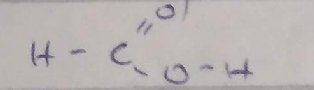
\includegraphics[width=.9\linewidth]{/home/shayan/Documents/org/notes/school/O3/chemistry/images/fig9.png}
\end{center}\\
Ethanoic Acid & \(CH_3COOH\) & \begin{center}
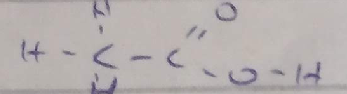
\includegraphics[width=.9\linewidth]{/home/shayan/Documents/org/notes/school/O3/chemistry/images/fig10.png}
\end{center}\\
Propanoic Acid & \(C_2H_5COOH\) & \begin{center}
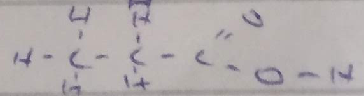
\includegraphics[width=.9\linewidth]{/home/shayan/Documents/org/notes/school/O3/chemistry/images/fig11.png}
\end{center}\\
Butanoic Acid & \(C_3H_7COOH\) & \begin{center}
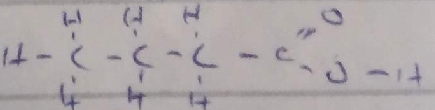
\includegraphics[width=.9\linewidth]{/home/shayan/Documents/org/notes/school/O3/chemistry/images/fig12.png}
\end{center}\\
\ldots{} & \ldots{} & \ldots{}\\
\end{tabular}
\end{center}
\begin{enumerate}
\item Chemical reactions
\label{sec:org4599691}
\begin{enumerate}
\item With water
\begin{itemize}
\item Carboxylic acids dissolve in water \& partially ionize to produce 1 hydrogen ion (\(H^+\)). For e.g.,
\begin{itemize}
\item \(HCOOH\) \(\frac{H_2O}{-->}\) \(H^+ + HCOO^-\) (methanoate)
\item \(CH_3COOH\) \(\frac{H_2O}{-->}\) \(H^+ CH_3COO\) (ethanoate)
\item \(C_2H_5COOH\) \(\frac{H_2O}{-->}\) \(H^+ C_2H_5COO\) (propanoate)
\end{itemize}
\end{itemize}
\item With bases
\begin{itemize}
\item Acid + base --> Salt + water
\begin{itemize}
\item \(CH_3COOH + Ca(OH)_2\) --> \(Ca(CH_3COO)_2\ (calcium\ ethanoate)\ + H_2O\)
\item \(C_2H_5COOH + NaOH\) --> \(NaC_2H_5COO\ (sodium\ propanoate)\ + H_2O\)
\end{itemize}
\end{itemize}
\item With carbonates
\begin{itemize}
\item Acid + carbonate --> Salt + water + carbon dioxide
\begin{itemize}
\item \(HCOOH + CaCO_3\) --> \(Ca(HCOO)_2 + H_2O + CO_2\)
\item \(CH_3COOH + K_2CO_3\) --> \(KCH_3COO + H_2O + CO_2\)
\item \(C_2H_5COOH + Na_2CO_3\) --> \(Na_2C_2H_5 + H_2O + CO_2\)
\end{itemize}
\end{itemize}
\item With metals
\begin{itemize}
\item Acid + metal --> Salt + hydrogen gas
\begin{itemize}
\item \(Zn + CH_3COOH\) --> \(Zn(CH_3COO)_2 + H_2\)
\item \(Mg + HCOOH\) --> \(MgHCOO + H_2\)
\end{itemize}
\end{itemize}
\end{enumerate}
\end{enumerate}
\subsubsection{Structured formulas}
\label{sec:org56c2cfd}
Structured formulas represent the structure of a compound.
\begin{itemize}
\item \begin{center}
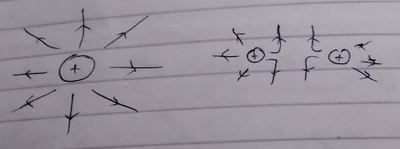
\includegraphics[width=.9\linewidth]{/home/shayan/Documents/org/notes/school/O3/chemistry/images/fig1.png}
\end{center}
\item \begin{center}
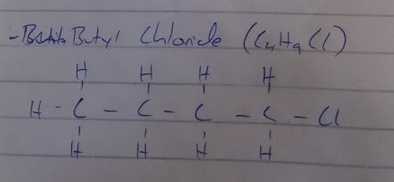
\includegraphics[width=.9\linewidth]{/home/shayan/Documents/org/notes/school/O3/chemistry/images/fig2.png}
\end{center}
\item \begin{center}
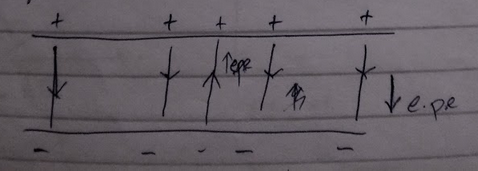
\includegraphics[width=.9\linewidth]{/home/shayan/Documents/org/notes/school/O3/chemistry/images/fig3.png}
\end{center}
\item \begin{center}
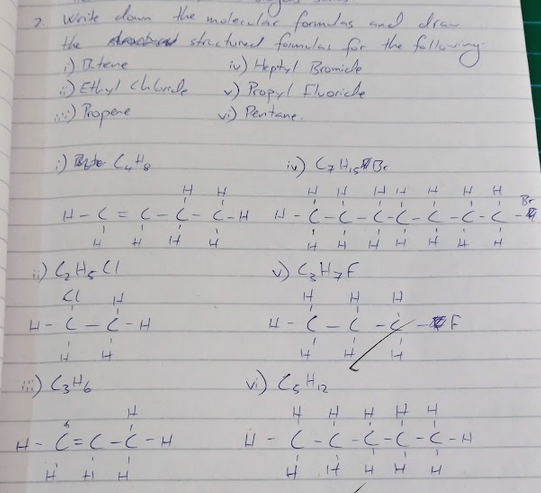
\includegraphics[width=.9\linewidth]{/home/shayan/Documents/org/notes/school/O3/chemistry/images/fig4.png}
\end{center}
\item \begin{center}
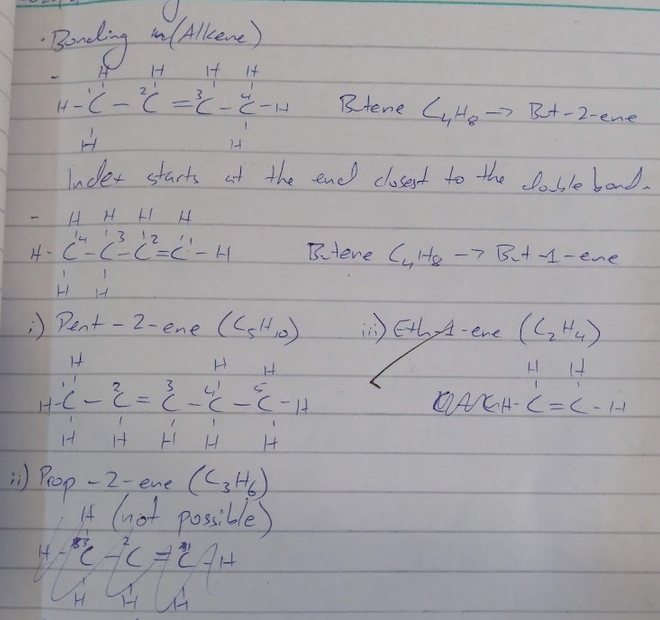
\includegraphics[width=.9\linewidth]{/home/shayan/Documents/org/notes/school/O3/chemistry/images/fig5.png}
\end{center}
\item \begin{center}
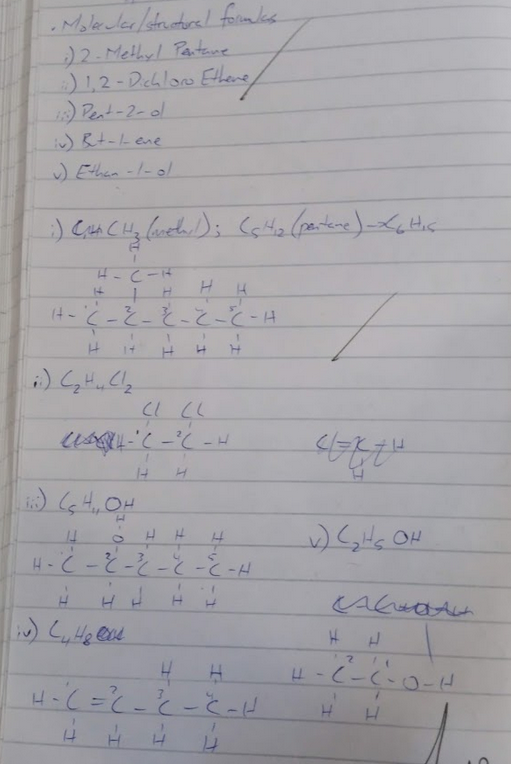
\includegraphics[width=.9\linewidth]{/home/shayan/Documents/org/notes/school/O3/chemistry/images/fig6.png}
\end{center}
\item \begin{center}
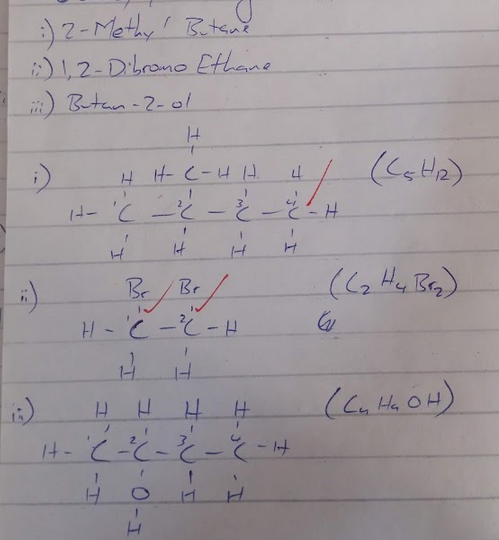
\includegraphics[width=.9\linewidth]{/home/shayan/Documents/org/notes/school/O3/chemistry/images/fig7.png}
\end{center}
\end{itemize}
\subsubsection{Esters}
\label{sec:org213587d}
Esters are formed when a mixture of alcohol and carboxylic acid is heated. The products formed are an alkyl alkanoate along with water.
\begin{enumerate}
\item Naming
\label{sec:org63c203a}
There are two parts to the name of an ester:
\begin{enumerate}
\item Alcohol
\item Carboxylic Acid
\end{enumerate}
For e.g.,
\begin{center}
\begin{tabular}{rllll}
 & Alcohol & Carboxylic Acid & Products & Chemical Equation\\
\hline
1. & Ethanol & Ethanoic Acid & Ethyl Ethanoate and Water & \(C_2H_5OH + CH_3COOH --> C_2H_5CH_3COO + H_2O\)\\
2. & Methanol & Methanoic Acid & Methyl Methanoate and Water & \(CH_3OH + HCOOH --> CH_3COO + H_2O\)\\
3. & Ethanol & Methanoic Acid & Ethyl Methanoate and Water & \(C_2H_5OH + HCOOH --> C_2H_5COO + H_2O\)\\
\end{tabular}
\end{center}
\item Structure
\label{sec:org148cb06}
\begin{enumerate}
\item Methyl Ethanoate (Ethanoic Acid + Methanol)
\end{enumerate}
\begin{center}
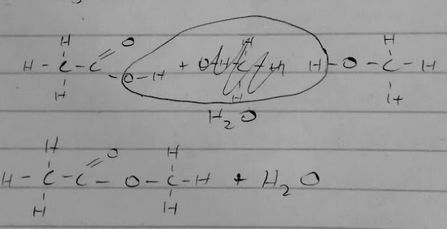
\includegraphics[width=.9\linewidth]{/home/shayan/Documents/org/notes/school/O3/chemistry/images/fig13.png}
\end{center}
\begin{enumerate}
\item Ethyl Methanoate (Methanoic Acid + Ethanol)
\end{enumerate}
\begin{center}
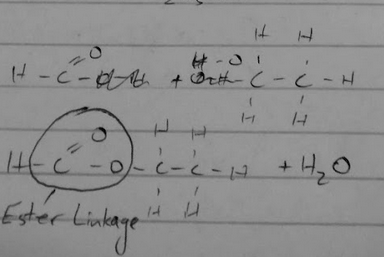
\includegraphics[width=.9\linewidth]{/home/shayan/Documents/org/notes/school/O3/chemistry/images/fig14.png}
\end{center}
\begin{enumerate}
\item Ethyl Ethanoate (Ethanoic Acid + Ethanol)
\end{enumerate}
\begin{center}
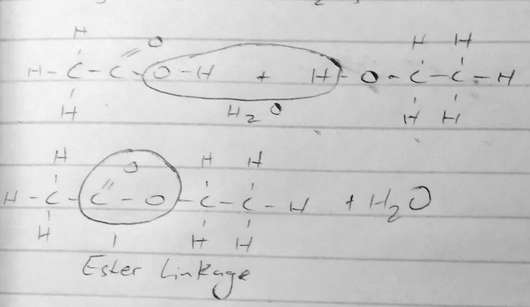
\includegraphics[width=.9\linewidth]{/home/shayan/Documents/org/notes/school/O3/chemistry/images/fig15.png}
\end{center}
\begin{enumerate}
\item Ester linkage
\label{sec:org160a64e}
An ester linkage is \(O=C-O-H\). The carbon bonds in an ester linkage are incomplete (3 of 4).
\end{enumerate}
\item Uses of esters
\label{sec:org491de88}
\begin{enumerate}
\item Artificial flavouring (courtesy of its fragrance)
\item Solvents (in cosmetics, perfumes, glue, etc)
\item Production of soaps (when fats are boiled with sodium hydroxide)
\end{enumerate}
\end{enumerate}
\subsection{Isomers}
\label{sec:orga0d604f}
Compounds which have the same molecular formula but different structural formulas are known as isomers.
\begin{center}
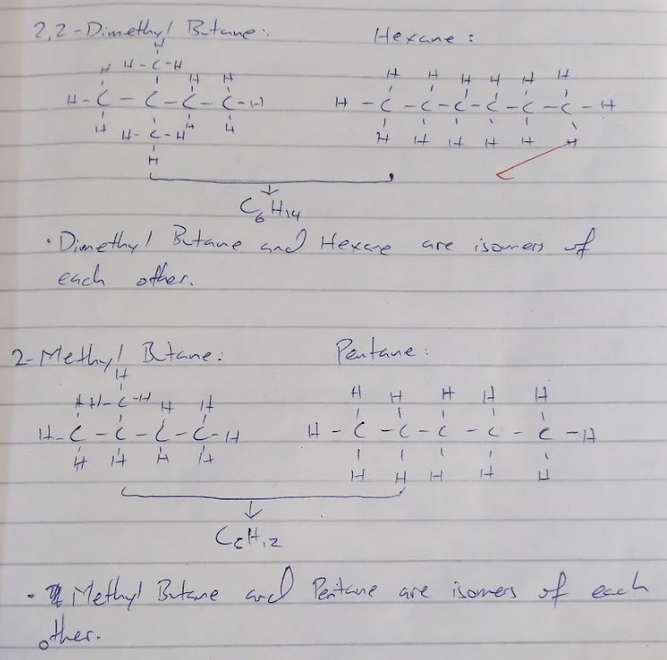
\includegraphics[width=.9\linewidth]{/home/shayan/Documents/org/notes/school/O3/chemistry/images/fig8.png}
\end{center}
\subsection{Fractional distillation of petroleum}
\label{sec:org64d8ec4}
Petroleum is a naturally-occuring liquid mixture of hydrocarbons, that is dark-brown in colour, has a high viscosity and is foul-smelling. In its unrefined form, petroleum is known as crude oil. In order for it to be used, it has to be refined first. This refining is done via fractional distillation.
\subsubsection{Process}
\label{sec:org5f9f30f}
\begin{enumerate}
\item In its raw form, petroleum is heated and vapourised.
\item The vapours are passed into the fractionating column.
\item The vapours rise up the fractionating column. The fractionating column is made up of a series of shelfs of varying temperatures. The lower shelves have a high temperature, the higher shelves have a lower temperature. When the vapours meet a shelf that is lower in temperature than its boiling point, it condenses and is collected.
\end{enumerate}
\subsubsection{Fractions}
\label{sec:org8bcd731}
A total of 7 fractions are collected from this process:
\begin{enumerate}
\item Petroleum gas
\item Gasoline
\item Naptha
\item Kerosene
\item Diesel
\item Lubricating oil
\item Bitumen
\end{enumerate}
\begin{enumerate}
\item Uses
\label{sec:org865959e}
\begin{enumerate}
\item Petroleum gas
\begin{itemize}
\item Used as fuel for cooking/heating.
\end{itemize}
\item Gasoline
\begin{itemize}
\item Used as a fuel for vehicles.
\end{itemize}
\item Naptha
\begin{itemize}
\item Used in the production of petrochemicals, i.e. plastics and detergents.
\end{itemize}
\item Kerosene
\begin{itemize}
\item Used as a fuel for aircrafts.
\end{itemize}
\item Diesel
\begin{itemize}
\item Used as a fuel for diesel engines in buses, lorries and trains.
\end{itemize}
\item Lubricating oil
\begin{itemize}
\item Used to lubricate machines/produce waxes + polishes.
\end{itemize}
\end{enumerate}
\end{enumerate}
\subsection{Polymers/Polymerization}
\label{sec:org5af9d56}
A polymer is a long-chain molecule, made up of repeat units known as monomers.
\subsubsection{Types of polymerization}
\label{sec:org06c062f}
\begin{enumerate}
\item Addition polymerization
\begin{itemize}
\item E.g.,
\begin{itemize}
\item polythene
\item PVC (poly-vinyl chloride)
\item teflon
\item polystyrene
\end{itemize}
\end{itemize}
\item Condensation polymerization
\begin{itemize}
\item E.g.,
\begin{itemize}
\item nylon (polyamide)
\item terylene (polyester)
\end{itemize}
\end{itemize}
\end{enumerate}
\begin{center}
\begin{tabular}{ll}
Addition polymerization & Condensation polymerization\\
\hline
Same monomer & Different monomer\\
No secondary substance is formed & Water is formed\\
\end{tabular}
\end{center}
\subsubsection{Addition polymerization}
\label{sec:org20fe7a2}
\begin{enumerate}
\item Structures
\label{sec:org8eb6cb8}
\begin{itemize}
\item \begin{center}
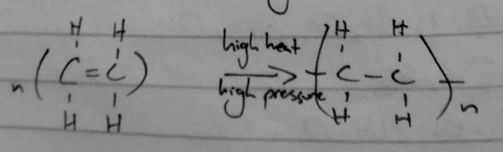
\includegraphics[width=.9\linewidth]{/home/shayan/Documents/org/notes/school/O3/chemistry/images/fig16.png}
\end{center}
\item \begin{center}
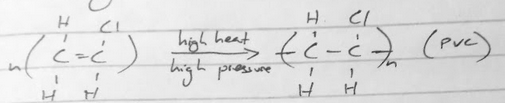
\includegraphics[width=.9\linewidth]{/home/shayan/Documents/org/notes/school/O3/chemistry/images/fig17.png}
\end{center}
\item \begin{center}
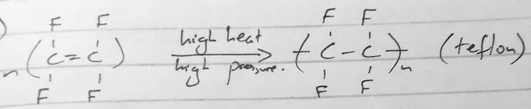
\includegraphics[width=.9\linewidth]{/home/shayan/Documents/org/notes/school/O3/chemistry/images/fig18.png}
\end{center}
\item \begin{center}
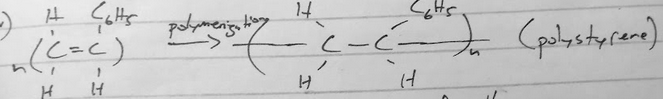
\includegraphics[width=.9\linewidth]{/home/shayan/Documents/org/notes/school/O3/chemistry/images/fig19.png}
\end{center}
\end{itemize}
\item Uses
\label{sec:orgfc8304e}
\begin{enumerate}
\item Polythene
\label{sec:orgc744ea7}
\begin{itemize}
\item Plastic products, e.g.,
\begin{itemize}
\item Clingfilm
\item Plastic bags
\item Buckets
\item Plastic toys
\end{itemize}
\end{itemize}
\item PVC
\label{sec:org55bf2ab}
\begin{itemize}
\item Pipes
\item Raincoats
\item Thin gloves
\item Flooring mats
\end{itemize}
\item Teflon
\label{sec:org2ade443}
\begin{itemize}
\item Non-stick frying pans
\end{itemize}
\item Polystyrene
\label{sec:org8009d75}
\begin{itemize}
\item Disposable containers
\end{itemize}
\end{enumerate}
\end{enumerate}
\subsubsection{Condensation polymerization}
\label{sec:org7c9af24}
\begin{enumerate}
\item Linkages
\label{sec:org638b7d9}
There are two linkages with condensed polymers:
\begin{itemize}
\item Ester linkages (\(O=C-O-\) (carbon bonds are 3 of 4))
\item Amide linkages (\(O=C-N-H\) (carbon bonds are 3 of 4))
\end{itemize}
\item Ester linkage
\label{sec:org9bb2db9}
Formed from Di-carboxylic acid + Di-alcohol (diol) and yields a polyester and water.
\begin{center}
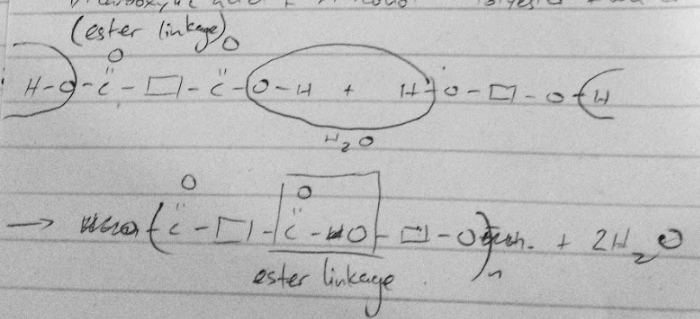
\includegraphics[width=.9\linewidth]{/home/shayan/Documents/org/notes/school/O3/chemistry/images/fig20.png}
\end{center}
\item Amide linkage
\label{sec:org35509c5}
Formed from Di-carboxylic acid + Di-amide and yields a polyamide and water.
\begin{center}
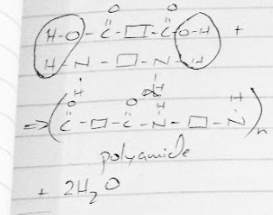
\includegraphics[width=.9\linewidth]{/home/shayan/Documents/org/notes/school/O3/chemistry/images/fig21.png}
\end{center}
\end{enumerate}
\subsubsection{Natural polymers}
\label{sec:org38ca999}
\begin{enumerate}
\item Protein
\label{sec:org38ff24b}
\begin{itemize}
\item Made of amino acids (being the monomers of protein)
\item Can be separated via chromatography (with ninhydrin as locating agent)
\end{itemize}
\begin{enumerate}
\item Structure of amino acids
\label{sec:orgc22ca33}
\begin{center}
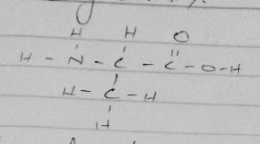
\includegraphics[width=.9\linewidth]{/home/shayan/Documents/org/notes/school/O3/chemistry/images/fig23.png}
\end{center}
\begin{itemize}
\item An amino acid is made up of a carbon atom bonded with:
\begin{enumerate}
\item The amine functional group, (\(NH_2\))
\item Hydrogen
\item An alkyl
\item The carboxylic acid functional group, (\(COOH\))
\end{enumerate}
\end{itemize}
\item Formation of proteins via condensation polymerization
\label{sec:orgdbfb8dc}
\begin{center}
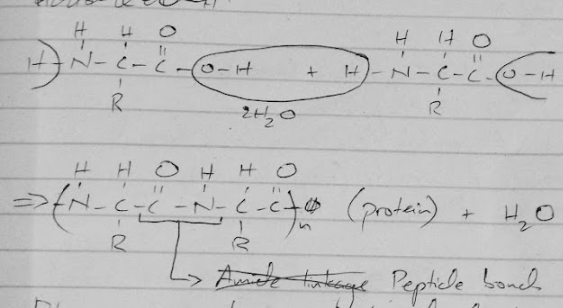
\includegraphics[width=.9\linewidth]{/home/shayan/Documents/org/notes/school/O3/chemistry/images/fig22.png}
\end{center}
\begin{itemize}
\item The linkage is \textbf{not} the amide linkage. Though it is the same, in a protein, this linkage is called a \textbf{peptide link}.
\item Because this is condensation polymerization, water is formed.
\end{itemize}
\end{enumerate}
\end{enumerate}
\section{Moles}
\label{sec:org40ce37b}
\subsection{Formulas}
\label{sec:orgd7958e2}
\subsubsection{Moles <-> Mass}
\label{sec:orgb77735e}
\(Mole = \frac{Mass(grams)}{Ar\ or\ Mr}\)
\subsubsection{Moles <-> Particles}
\label{sec:org9212ceb}
\(Mole = \frac{Total\ number\ of\ particles}{6*10^{23}\ (Avogadro's\ Number)}\)
\subsubsection{Moles <-> Volume of gas}
\label{sec:org839b506}
\(dm^3\) --> \(cm^3\) = \(*1000\)
\(cm^3\) --> \(dm^3\) = \(/1000\)
\begin{enumerate}
\item \(dm^3\)
\label{sec:org99dd7f8}
\(Mole = \frac{Volume\ of\ gas\ (dm^3)}{24}\)
\item \(cm^3\)
\label{sec:org878e299}
\(Mole = \frac{Volume\ of\ gas\ (cm^3)}{24000}\)
\end{enumerate}
\subsubsection{Moles <-> Concentration}
\label{sec:orgec79905}
\begin{enumerate}
\item \(g/dm^3\)
\label{sec:org6aa05f4}
\(Concentration = \frac{Mass\ of\ solute}{Volume\ of\ solution}\)
\item \(mol/dm^3\)
\label{sec:orga3f03bf}
\(Concentration = \frac{Moles\ of\ solute}{Volume\ of\ solution}\)
\end{enumerate}
\section{Electrolysis}
\label{sec:org692cfc0}
\subsection{Key points}
\label{sec:org932c055}
\begin{enumerate}
\item Ions
\item Selective discharge
\item Concentration of elecrolyte
\item Nature of electrodes
\item Reactions at anode and cathode
\item Changes in electrolyte
\item Identification
\item Diagrams
\end{enumerate}
\subsection{Basic Terms}
\label{sec:org459dcb2}
\subsubsection{Ions}
\label{sec:orgd5aefd2}
A particle with a positive or negative charge.
\begin{itemize}
\item Anions are negatively charged ions.
\item Cations are positively charged ions.
\end{itemize}
\subsubsection{Electrodes}
\label{sec:org73ccfd4}
A metal/non-metal (i.e. graphite) that conducts electricity.
Anions(-) --> Anode($\backslash$+); Cations(+)--> Cathode(-)
\begin{itemize}
\item Anodes
Positively charged electrode
\item Cathode
Negatively charged electrode
\end{itemize}
\subsubsection{Ionization}
\label{sec:org5b8da8d}
The process by which a particle is positively or negatively charged.
\subsubsection{Redox}
\label{sec:org8a887d8}
A chemical reaction involving the oxidation/reduction of elements.
\begin{itemize}
\item Oxidation
A rise in the oxidation state
\item Reduction
A decrease in the oxidation state
\end{itemize}
\subsubsection{Electrochemical cells}
\label{sec:org457fc1b}
An electrolytic cell that handled electrical and chemical energy.
\begin{itemize}
\item Simple/Volatic cell
Chemical energy --> electric energy
\item Electrolytic cell
Electric energy --> chemical energy
\end{itemize}
\subsubsection{Electrolytes}
\label{sec:orge66f7dc}
An ionic compound (fused/aqueous) that conducts electricity, thereby forming anions and cations.
\begin{itemize}
\item Strong electrolytes
Easily conducts electricity
\item Weak electrolytes
Conducts electricity, but not as easily
\end{itemize}
\subsection{Simple cells vs electrochemical cells}
\label{sec:orgea43e21}
\subsubsection{Simple cells}
\label{sec:org3932770}
\begin{itemize}
\item Chemical energy --> electric energy
\item Spontaneous reaction
\end{itemize}
\subsubsection{Electrochemical cells}
\label{sec:org02857be}
\begin{itemize}
\item Electric energy --> chemical energy
\item Non-spontaneous reaction
\end{itemize}
\subsection{Selective discharge}
\label{sec:org86f2e3a}
\subsubsection{Selective discharge of anions}
\label{sec:org5d46af3}
Ease of discharge increases down the group, i.e. \#9 has preference over \#1 when it comes to discharging at the anode.
\begin{enumerate}
\item Potassium ion, \(K^+\)
\item Sodium ion, \(Na^+\)
\item Calcium ion, \(Ca^{2+}\)
\item Magnesium ion, \(Mg^{2+}\)
\item Zinc ion, \(Zn^{2+}\)
\item Lead ion, \(Pb^{2+}\)
\item Hydrogen ion, \(H^+\)
\item Copper(II) ion, \(Cu^{2+}\)
\item Silver ion, \(Ag^+\)
\end{enumerate}
\subsubsection{Selective discharge of cations}
\label{sec:org20cc1e7}
Ease of discharge increases down the group, i.e. \#6 has preference over \#1 when it comes to discharging at the cathode.
\begin{enumerate}
\item Sulfate ion, \(SO_4^{2-}\)
\item Nitrate ion, \(NO_3^-\)
\item Chloride ion, \(Cl^-\)
\item Bromide ion, \(Br^-\)
\item Iodide ion, \(I^-\)
\item Hydroxide ion, \(OH^-\)
\end{enumerate}
\subsection{Concentration of electrolyte}
\label{sec:orgf9078d6}
The concentration of the electrolyte should be kept in mind, since different levels of concentration yield different results.
\begin{center}
\begin{tabular}{lllll}
 & Ions & Reaction at anode & Reaction at cathode & Change in electrolyte\\
\hline
Sodium Chloride (aq) & \(Na^+, Cl^-, H^+, OH^-\) & \(4OH^- --> 4e^- (aq) + H_2O (l) + O_2 (g)\) & \(2H^+ + 2e^- --> H_2 (g)\) & Concentration of \(NaCl\) increases\\
Sodium Chloride (concentrated) & \(Na^+, Cl^-, H^+, OH^-\) & \(2Cl^- --> 2e^- (aq) + Cl_2 (s)\) & \(2H^+ + 2e^- --> H_2 (g)\) (because sodium reacts with \(OH\) before it can be discharged) & \(NaOH\) forms, turning the electrolyte alkaline\\
\end{tabular}
\end{center}
\subsection{Nature of electrodes}
\label{sec:org02229fa}
The material of the electrode can yield different results. A reactive electrode may partake in the process of electrolysis, while an unreactive electrode does not.
\subsection{Reaction at anode and cathode}
\label{sec:org93318ac}
\subsubsection{Anode}
\label{sec:orgd2adf1d}
Oxidation occurs at the anode.
\subsubsection{Cathode}
\label{sec:org590abf7}
Reduction occurs at the cathode.
\subsection{Changes in electrolyte}
\label{sec:org4a4dd48}
Possible changes to an electrolyte after electrolysis include:
\begin{enumerate}
\item Concentration
\begin{itemize}
\item The concentration of solute in the electrolyte may change after electrolysis has occurred. Take the electrolysis of Sodium Chloride (aq):
\begin{enumerate}
\item Ions
\begin{itemize}
\item \(Na^+, Cl^-, H^+, OH^-\)
\end{itemize}
\item Reaction at anode
\begin{itemize}
\item \(4OH^- --> 4e^- (aq) + H_2O (l) + O_2 (g)\)
\end{itemize}
\item Reaction at cathode
\begin{itemize}
\item \(2H^+ + 2e^- --> H_2 (g)\)
\end{itemize}
\item Change in electrolyte
\begin{itemize}
\item Since hydrogen and water are released in the form of gas, the elements left in the electrolyte are sodium chloride and an amount of water, less than before. This means the concentration of sodium chloride has increased after electrolysis.
\end{itemize}
\end{enumerate}
\end{itemize}
\item Colour
\begin{itemize}
\item The colour of an electrolyte may change after electrolysis. In the case of copper sulfate, for example, the electrolyte turns from blue to colourless.
\end{itemize}
\item Acidity
\begin{itemize}
\item If a compound with hydrogen forms, i.e. \(HCl\) or \(H_2SO_4\), the electrolyte has turned acidic.
\end{itemize}
\item Alkalinity
\begin{itemize}
\item If a compound with hydroxide forms, i.e. \(NaOH\) or \(KOH\), the electrolyte has turned alkaline.
\end{itemize}
\end{enumerate}
\subsection{Identification of products}
\label{sec:org3bcd6b7}
Refer to \ref{sec:org131db2f}
\section{Metals}
\label{sec:orgaba8250}
\subsection{Extraction of metals}
\label{sec:org256dfe0}
\begin{enumerate}
\item Ores
\label{sec:orgf203b7f}
An ore is a mineral that contains a sufficient quantity of metal(s) that can be easily extracted.
\end{enumerate}
\subsubsection{Extraction}
\label{sec:orgea298ea}
\begin{enumerate}
\item Reactive metals
\label{sec:org04ce976}
Reactive metals are separated via electrolysis. For e.g.,
\begin{itemize}
\item \(Al_2O_3 --> Al^{3_}+O^{2-}\)
\end{itemize}
\item Unreactive metals
\label{sec:org5eb668c}
Unreactive metals are separated via reduction. For e.g.,
\begin{itemize}
\item \(PbO + C \frac{heat}{-->} Pb + CO\)
\item \(ZnO + C \frac{heat}{-->} Zn + CO\)
\end{itemize}
\end{enumerate}
\item Extraction of iron
\label{sec:org39ef8e4}
\begin{enumerate}
\item Outline
\label{sec:org02668cf}
\begin{enumerate}
\item Ore
\item Diagram labeling (blast furnace)
\item Rise/fall in temperature
\item Type of reaction (exothermic/endothermic)
\item Removal of impurities (slag formation)
\item Extraction of iron
\end{enumerate}
\end{enumerate}
\end{enumerate}
\section{Air, water and gases}
\label{sec:orgde844e1}
\subsection{Treatment of water}
\label{sec:org7df6626}
\subsubsection{Filtration}
\label{sec:org284e419}
Water is pumped out through filters to trap any large particles.
\begin{enumerate}
\item Natural filtration
\label{sec:orgb0c0fcd}
Water is passed through a bed of sand (which is insoluble in water), acting as a natural filter.
\end{enumerate}
\subsubsection{Coagulation}
\label{sec:orgd25ddcc}
A coagulant (i.e. \(Fe_2(SO_4)_3\) (Iron(III) sulfate)) is added to the water to make small, suspended particles stick together. Air is then blown through the water to make the coagulated particles rise to the top of the water in the form of froth/foam.
\subsubsection{Purification}
\label{sec:org1f5cb35}
\begin{enumerate}
\item Charcoal
\label{sec:org8269c83}
Charcoal can be used to remove the taste and smell of water.
\item Chlorination
\label{sec:org61d4e7b}
Chlorine is added to kill the bacteria and some other microbes in the water.
\end{enumerate}
\subsection{Fertilizers}
\label{sec:org28828d6}
Most fertilizers are made from:
\begin{enumerate}
\item nitrogen (for the chlorophyll and protein of plants)
\item phosphorous (for the roots of a plant and the ripening of fruits)
\item potassium (for the protein of plants)
\end{enumerate}
\subsection{Ammonia}
\label{sec:org228bbda}
\subsubsection{Industrial preparation of Ammonia (\(NH_3\))}
\label{sec:org40b56a4}
\begin{enumerate}
\item Raw materials
\label{sec:orge5474cd}
In order to make ammonia on an industrial scale, the following is needed:
\begin{enumerate}
\item Hydrogen
\begin{itemize}
\item Obtained via:
\begin{enumerate}
\item cracking of alkanes
\item reacting methane with steam
\end{enumerate}
\end{itemize}
\item Nitrogen
\begin{itemize}
\item Obtained via:
\begin{enumerate}
\item fractional distillation of air
\end{enumerate}
\end{itemize}
\end{enumerate}
\end{enumerate}
\subsubsection{Haber's process}
\label{sec:org0066bec}
\begin{enumerate}
\item Chemical reaction
\label{sec:org3c3d4c4}
\begin{itemize}
\item \(N_2+3H_2 \frac{Fe, 200atm, 450°C}{<-->}2NH_3\) (reversible)
\end{itemize}
\begin{enumerate}
\item Conditions
\label{sec:org7280bfa}
\begin{enumerate}
\item 450°C (temperature)
\item 200atm (pressure)
\item Iron (catalyst)
\end{enumerate}
\end{enumerate}
\end{enumerate}
\end{document}
